\section*{Revisjonshistorie}
\begin{center}
 \begin{tabular}{|p{1.5cm} p{5.5cm}|} 
 \hline
 År & Forfatter \\ [0.5ex] 
 \hline\hline
 2020 & Kolbjørn Austreng  \\ 
 \hline
 2021 & Kiet Tuan Hoang \\
 \hline
  2022 & Kiet Tuan Hoang \\
 \hline
   2023 & Kiet Tuan Hoang \\
 \hline
\end{tabular}
\end{center}

\begin{alphasection}
\section{Introduksjon - Praktisk rundt filene}

I denne øvingen får dere ikke utlevert noen \verb|.c| eller \verb|.h|-filer.


\section{Introduksjon - Praktisk rundt øvingen}
Versjonskontroll er en måte å ta \textit{bilder} av en fil, slik at man kan se hvordan filen har endret seg, og når endringene ble gjort. Programmet \verb|git| er et utbredt verktøy for versjonskontroll. Versjonskontroll er spesielt viktig når man jobber flere i lag på de samme filene.

Denne øvingen er ment som en introduksjon til praktisk bruk av \verb|git|. For å illustrere de mest brukte delene av \verb|git| vil øvingen være strukturert som en walkthrough og består av å skrive enkel \verb|C|-kode, som skal versjonskontrolleres (introduksjon \ref{sec:innføring}). Oppgaven finner dere i seksjon \ref{sec:2-oppgave} og handler om at dere skal vise at dere mestrer \verb|git| til en studass for å få godkjent øvingen.

\subsection{Avhengigheter}

Denne øvingen krever at man har \verb|git| på datamaskinen før man begynner. Datamaskinene på Sanntidssalen har \verb|git| installert, men det kan også være greit å skaffe det selv også, ettersom det er et nyttig verktøy. Dette kan gjøres via \href{https://git-scm.com/downloads}{https://git-scm.com}, eller via en pakkebehandler om operativsystemet har en\footnote{apt, yum, pacman etc for Linux. Homebrew for mac}.

I tillegg til \verb|git|, trenger man en \verb|C|-kompilator og tekstbehandler for å kompilere og skrive \verb|C|-kodene vi kommer til å versjonskontrollere. Denne oppgaveteksten kommer til å bruke \verb|gcc|, men en hvilken som helst \verb|C|-kompilator vil fungere (datamaskinene på Sanntidssalen har allerede \verb|gcc| installert).


\section{Introduksjon - Grunnleggende Kommandoer}\label{sec:innføring}

\subsection{Oppsett}

Åpne en terminal og skriv inn \verb|git --version|. Dette er en enkel test for å sjekke om \verb|git| er riktig installert og ligger i \verb|PATH|-variabelen til operativsystemet.


Før \verb|git| kan brukes må man gjøre noen enkle konfigurasjoner. Først og fremst må \verb|git| har litt informasjon om brukeren. Dette må bare gjøres en gang, og består av to kommandoer:

\begin{lstlisting}[mathescape=true]
student@Ubuntu:$\smallsim$$\verb|$|$ git config --global user.name "Kiet Tuan Hoang"
student@Ubuntu:$\smallsim$$\verb|$|$ git config --global user.email "kietth@stud.ntnu.no"
\end{lstlisting}


Flagget \verb|--global| fører til at \verb|git| lagrer navn og email i filen \texttt{$\smallsim$/.gitconfig}. Om man jobber på en datamaskin andre bruker - slik som i heisprosjektet, er det lurt å konfigurere \verb|git| lokalt. Det gjøres fra et allerede opprettet \verb|git|-repository, ved å kalle de samme kommandoene uten \verb|--global|-flagget:

\begin{lstlisting}[mathescape=true]
student@Ubuntu:$\smallsim$$\verb|$|$ git config user.name "Kiet Tuan Hoang"
student@Ubuntu:$\smallsim$$\verb|$|$ git config user.email "kietth@stud.ntnu.no"
\end{lstlisting}

For ekstra brukervennlighet, har \verb|git| muligheten til å definere aliaser for lange kommandoer som ofte brukes. For eksempel brukes kommandoen \verb|git checkout| ofte slik at mange liker å aliase denne til \verb|git co|. For denne øvingen definerer man aliaset \verb|lg| (betyr det samme som \verb|git log --all --oneline| \verb|--graph --decorate|):

\begin{lstlisting}[mathescape=true]
student@Ubuntu:$\smallsim$$\verb|$|$ git config --global alias.lg "log --all --oneline --graph --decorate"
\end{lstlisting}

Akkurat dette aliaset er spesielt nyttig for videre bruk av \verb|git|.




\subsection{\texttt{git init}}

\verb|git| er basert på at man har en \textit{oppbevaringsmappe} kalt repository. Om man ønsker å skrive kode i en mappe kalt \verb|demo|, og at \verb|git| skal følge med koden, kan man skrive følgende fra terminalen: 

\begin{lstlisting}[mathescape=true]
student@Ubuntu:$\smallsim$$\verb|$|$ mkdir demo
student@Ubuntu:$\smallsim$$\verb|$|$ cd demo
student@Ubuntu:$\smallsim$$\verb|$|$ git init

Initialized empty Git repository in /home/student/demo/.git/
\end{lstlisting}

\verb|mkdir| (\textit{\textbf{m}ake \textbf{dir}ectory}) vil opprette mappen \verb|demo|, og \verb|cd| (\textit{\textbf{c}hange \textbf{d}irectory}) vil flytte brukeren inn i den. Til slutt vil kommandoen \verb|git init| oprette en gjemt mappe med navn \verb|.git| inne i demo-mappen, som \verb|git| vil bruke for å holde styr på filene i mappen.

\subsection{\texttt{git status, git add, git commit}}


Dere har nå en tom \verb|git|-mappe (\verb|demo|). Kall kommandoen \verb|git status|. Hvis dere ikke har gjort noen endringer i mappen så langt, vil dere få tilbake en melding som dette:

\begin{lstlisting}[mathescape=true]
student@Ubuntu:$\smallsim$$\verb|$|$ git status

On branch master

No commits yet

nothing to commit (create/copy files and use "git add" to track)
\end{lstlisting}


Stort sett er \verb|git| veldig behjelpelig med å fortelle brukeren hva som foregår. Om man lurer på hva som skjer, er utskriften fra \verb|git| oftest et godt svar.

Opprett nå en fil kalt \verb|main.c| i demo-mappen, og skriv inn det følgende med en hvilken som helst tekstbehandler:

\begin{lstlisting}
#include <stdio.h>

int main(){
        return 0;
}
\end{lstlisting}

Dersom dere nå lagrer denne filen, og kjører \verb|git status| på nytt burde dere se noe slikt eller liknende avhengig av hvilken versjon av \verb|git| dere har:

\begin{lstlisting}[mathescape=true]
student@Ubuntu:$\smallsim$$\verb|$|$ git status

On branch master

No commits yet

Untracked files:
    (use "git add <file>..." to include in what will be committed)
           main.c

nothing added to commit but untracked files present (use "git add" to track)
\end{lstlisting}

Denne utskriften forteller oss at vi nå har en ny fil i \verb|demo|-mappen ved navn \verb|main.c|, som \verb|git| foreløpig ikke bryr seg om. Kall nå \verb|git add main.c|, etterfulgt av \verb|git status| for å få opp denne meldingen:

\begin{lstlisting}[mathescape=true]
student@Ubuntu:$\smallsim$$\verb|$|$ git add main.c
student@Ubuntu:$\smallsim$$\verb|$|$ git status

On branch master

No commits yet

Changes to be committed:
  (use "git rm --cached <file>..." to unstage)
	      new file:     main.c
\end{lstlisting}

Dette betyr at \verb|git| har lagt til \verb|main.c| i sitt \textit{staging area}, som er stedet før \verb|git| \textit{tar et bilde} av mappen. Dersom man nå skriver \verb|git commit -m "added main.c"| etterfulgt av \verb|git lg|\footnote{Dette er aliaset vi tidligere opprettet og defineres som \texttt{git log --all --oneline --graph --decorate}} vil man se noe slikt:

\begin{lstlisting}[mathescape=true]
student@Ubuntu:$\smallsim$$\verb|$|$ git commit -m "added main.c" 

[master (root-commit) 7cb84fb] added main.c
 1 file changed, 5 insertions(+)
 create mode 100644 main.c

student@Ubuntu:$\smallsim$$\verb|$|$ git lg

* 7cb84fb (HEAD -> master) added main.c
\end{lstlisting}




Det siste vi ser på denne linjen er en stjerne. Denne stjernen representerer et \textit{bilde} som \verb|git| har tatt for oss. De sju heksadesimale tallene som følger etter er et utsnitt av en hash på 40 bokstaver, som \verb|git| bruker for å identifisere \textit{bilder} (eller \textit{commits}). Denne hashen er spesielt viktig, om man vil inspisere tidligere \textit{bilder} som \verb|git| har lagret.

I parentesen står det (\verb|HEAD -> master|), som betyr at hodepekeren til \verb|git| peker på akkurat dette \textit{bildet}, som befinner seg på grenen \verb|master|. Til slutt står det \verb|added main.c| som er \textit{commit}-meldingen vi ga dette bildet, for å beskrive hva vi har gjort.


\subsection{Terminologi og \texttt{git}s indre}
Figur \ref{fig:2-oppgaveish} viser arbeidflyten som kan forventes med \verb|git|,


\begin{figure}[ht]
    \centering
    

\tikzset{every picture/.style={line width=0.75pt}} %set default line width to 0.75pt        

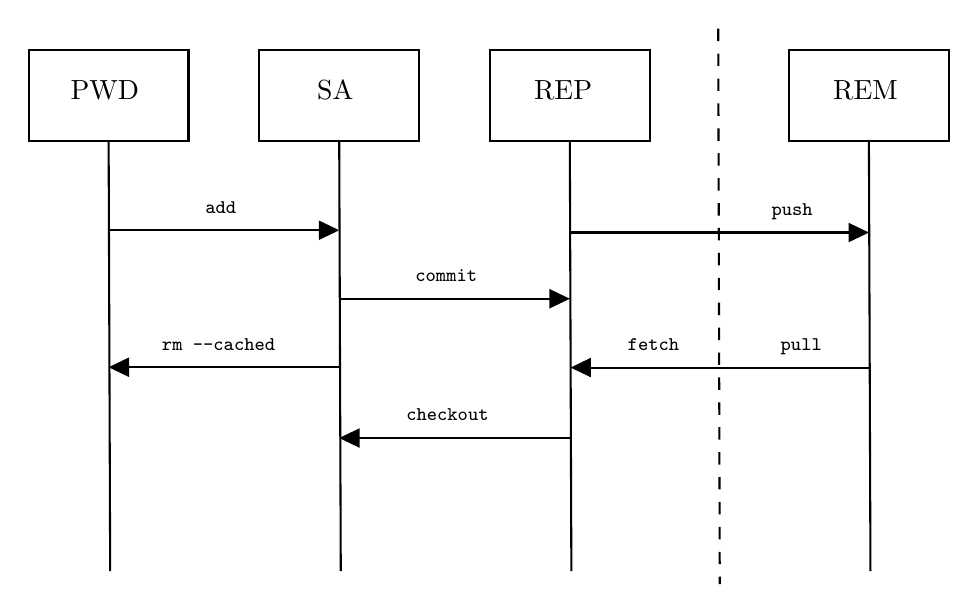
\begin{tikzpicture}[x=0.75pt,y=0.75pt,yscale=-1.1,xscale=1.1]
%uncomment if require: \path (0,300); %set diagram left start at 0, and has height of 300

%Shape: Rectangle [id:dp9926262498552592] 
\draw   (30,61) -- (100,61) -- (100,101) -- (30,101) -- cycle ;

%Straight Lines [id:da29368230412672536] 
\draw    (65,101) -- (65.68,289.27) ;

%Shape: Rectangle [id:dp08169817348503838] 
\draw   (131,61) -- (201,61) -- (201,101) -- (131,101) -- cycle ;

%Straight Lines [id:da14910629817767407] 
\draw    (166,101) -- (166.68,289.27) ;

%Shape: Rectangle [id:dp2040495981987429] 
\draw   (232,61) -- (302,61) -- (302,101) -- (232,101) -- cycle ;

%Shape: Rectangle [id:dp8791019060072369] 
\draw   (363,61) -- (433,61) -- (433,101) -- (363,101) -- cycle ;

%Straight Lines [id:da578357148806447] 
\draw    (267,101) -- (267.68,289.27) ;
%Straight Lines [id:da8146040086450574] 
\draw    (398,101) -- (398.68,289.27) ;
%Straight Lines [id:da3998430026566486] 
\draw    (65,140) -- (163,140) ;
\draw [shift={(166,140)}, rotate = 180] [fill={rgb, 255:red, 0; green, 0; blue, 0 }  ][line width=0.08]  [draw opacity=0] (8.93,-4.29) -- (0,0) -- (8.93,4.29) -- cycle    ;
%Straight Lines [id:da4617707088758103] 
\draw    (68,200) -- (166,200) ;
\draw [shift={(65,200)}, rotate = 0] [fill={rgb, 255:red, 0; green, 0; blue, 0 }  ][line width=0.08]  [draw opacity=0] (8.93,-4.29) -- (0,0) -- (8.93,4.29) -- cycle    ;
%Straight Lines [id:da4070062828946528] 
\draw    (166,170) -- (264,170) ;
\draw [shift={(267,170)}, rotate = 180] [fill={rgb, 255:red, 0; green, 0; blue, 0 }  ][line width=0.08]  [draw opacity=0] (8.93,-4.29) -- (0,0) -- (8.93,4.29) -- cycle    ;
%Straight Lines [id:da49432195113072197] 
\draw    (169,231) -- (267,231) ;
\draw [shift={(166,231)}, rotate = 0] [fill={rgb, 255:red, 0; green, 0; blue, 0 }  ][line width=0.08]  [draw opacity=0] (8.93,-4.29) -- (0,0) -- (8.93,4.29) -- cycle    ;
%Straight Lines [id:da2695146956164247] 
\draw  [dash pattern={on 4.5pt off 4.5pt}]  (332,51.73) -- (332.68,295) ;
%Straight Lines [id:da19896549823915888] 
\draw    (267,141) -- (395,141) ;
\draw [shift={(398,141)}, rotate = 180] [fill={rgb, 255:red, 0; green, 0; blue, 0 }  ][line width=0.08]  [draw opacity=0] (8.93,-4.29) -- (0,0) -- (8.93,4.29) -- cycle    ;
%Straight Lines [id:da6178333215153113] 
\draw    (270.34,200.14) -- (398.34,200.14) ;
\draw [shift={(267.34,200.14)}, rotate = 0] [fill={rgb, 255:red, 0; green, 0; blue, 0 }  ][line width=0.08]  [draw opacity=0] (8.93,-4.29) -- (0,0) -- (8.93,4.29) -- cycle    ;

% Text Node
\draw (47,73) node [anchor=north west][inner sep=0.75pt]   [align=left] {PWD};
% Text Node
\draw (155,73) node [anchor=north west][inner sep=0.75pt]   [align=left] {SA};
% Text Node
\draw (250,73) node [anchor=north west][inner sep=0.75pt]   [align=left] {REP};
% Text Node
\draw (381,73) node [anchor=north west][inner sep=0.75pt]   [align=left] {REM};
% Text Node
\draw (106,126) node [anchor=north west][inner sep=0.75pt]  [font=\scriptsize] [align=left] {\texttt{add}};
% Text Node
\draw (87,186) node [anchor=north west][inner sep=0.75pt]  [font=\scriptsize] [align=left] {\texttt{rm --cached}};
% Text Node
\draw (198,156) node [anchor=north west][inner sep=0.75pt]  [font=\scriptsize] [align=left] {\texttt{commit}};
% Text Node
\draw (194,217) node [anchor=north west][inner sep=0.75pt]  [font=\scriptsize] [align=left] {\texttt{checkout}};
% Text Node
\draw (354,127) node [anchor=north west][inner sep=0.75pt]  [font=\scriptsize] [align=left] {\texttt{push}};
% Text Node
\draw (358,186) node [anchor=north west][inner sep=0.75pt]  [font=\scriptsize] [align=left] {\texttt{pull}};
% Text Node
\draw (291,186) node [anchor=north west][inner sep=0.75pt]  [font=\scriptsize] [align=left] {\texttt{fetch}};


\end{tikzpicture}
    \caption{Arbeidsflyt i \texttt{git}.}
    \label{fig:2-oppgaveish}
\end{figure}
\newpage
hvor:

\begin{itemize}
    \item \textbf{PWD}: \textit{Current working directory}, dette er mappen som \verb|git| holder styr på.
    \item \textbf{SA}: \textit{Staging area}, her legges filer \verb|git| skal \textit{ta bilde av}, før de legges til i historikken.
    \item \textbf{REP}: \textit{Repository}, dette er all historien \verb|git| kjenner til. Bilder som er tatt av tidligere versjoner av filer legges til her, som en ny stjerne i en graf
    som representerer alt som har skjedd hittil.
    
    \item \textbf{REM}: \textit{Remote}, dette er stort sett en ekstern server (men kan være en annen
    lokal mappe), dit \verb|git| vil dytte lokale endringer, og ta endringer gjort
    av andre fra. 
\end{itemize}



Til nå har vi vært innom \textbf{PWD}, \textbf{SA}, og \textbf{REP} ved at vi har laget en enkel \verb|C|-kode (\verb|main.c|) som vi har tatt \textit{bilde} av med \verb|git|. Vi kommer ikke til å sette opp eksterne servere, så vi kommer ikke borti \textbf{REM}\footnote{I praksis brukes \href{https://github.com}{https://github.com} som ekstern server.}. For å få mer kunnskap om \verb|git|, skal vi nå bygge videre på den lokale \verb|git|-grafen vår.

\subsection{\texttt{git diff, git checkout}}

Endre \verb|main.c| til å inneholde dette:

\begin{lstlisting}
#include <stdio.h>

int main(){
        printf("Hello world\n");
        return 0;
}
\end{lstlisting}

Kjør deretter \verb|git status|. Dere vil nå se:

\begin{lstlisting}[mathescape=true]
student@Ubuntu:$\smallsim$$\verb|$|$ git status

On branch master

Changes not staged for commit:
  (use "git add <file>..." to update what will be committed)
  (use "git restore <file>..." to discard changes in working directory)
	      modified:    main.c

no changes added to commit (use "git add" and/or "git commit -a")
\end{lstlisting}


Dette forteller oss at \verb|git| vet at \verb|main.c| har endret seg, men fordi vi ikke har lagt den til i \textit{staging area}, vil ikke \verb|git| ta et bilde av den.

For å få en oversikt over hva som har endret seg siden sist, kan man bruke kommandoen \verb|git diff|. Dersom vi nå kaller \verb|git diff main.c| vil vi få:

\begin{lstlisting}[mathescape=true]
student@Ubuntu:$\smallsim$$\verb|$|$ git diff main.c

@@ -1,5 + 1,6 @@
 #include <stdio.h>\newline
 int main(){
+        printf("Hello world\n");
         return 0;
}
\end{lstlisting}



hvor et pluss-tegn representerer en linje som har blitt lagt til, mens et minus-tegn representerer en linje som har blitt tatt bort. \verb|git diff| er spesielt viktig dersom man har gjort mange endringer på en gang, og ikke husker hva man har gjort.

Dersom dere nå kjører \verb|git add main.c| og \verb|git commit -m "classic|  \verb|example code"|, etterfulgt av \verb|git lg| vil dere se:

\begin{lstlisting}[mathescape=true]
student@Ubuntu:$\smallsim$$\verb|$|$ git add main.c
student@Ubuntu:$\smallsim$$\verb|$|$ git commit -m "classic example code"

[master df7e5b2] classic example code
 1 file changed, 1 insertion(+)

student@Ubuntu:$\smallsim$$\verb|$|$ git lg

* df7e5b2 (HEAD -> master) classic example code
* 7cb84fb added main.c
\end{lstlisting}


Dette betyr at vi nettopp tok et nytt bilde av \verb|main.c|, og at vi la denne
til øverst i \textit{historikktreet}. Den \textit{gamle} koden som ikke gjorde noe ligger
fortsatt i \verb|git|s minne (med hashen \verb|7cb84fb|), men grenen kalt \verb|master| (og også vår hodepeker)
peker til den nye \verb|printf|-koden vi akkurat skrev som har fått hashen \verb|df7e5b2|.

Det som gjør \verb|git| veldig nyttig er at det er mulig å få tidligere \textit{bilder}, ved å hoppe tilbake i historikk-grafen. Dersom dere nå kjører \verb|git checkout 7cb84fb|\footnote{Hashsummen deres kan være annerledes enn oppgaveteksten. Hashen til den gamle koden kan fås ved å kjøre \texttt{git lg}.} vil dere få en melding som sier at dere er i \verb|detached HEAD state|. Her kan man leke med den gamle koden som \verb|git| har tatt vare på. Om man nå kaller \verb|git checkout master| kommer man tilbake til den nye koden.


\subsection{\texttt{git branch, git merge}}

Når dere jobber på samme kodebase, kommer versjonskonflikter til å oppstå. Dette kan lett bli håndtert med \verb|git branch| og \verb|git merge|.

Kall først \verb|git branch other|, etterfulgt av \verb|git checkout other|. Dette vil lage en ny gren, kalt \verb|other|, og hoppe til den. Denne grenen skal simulere at dere er to som jobber på samme kode. Dette er så vanlig at \verb|git | har en innebygd kommando for akkurat dette: \verb|git checkout -b <grennavn>|.

Om dere nå kaller \verb|git lg|, vil dere se følgende:

\begin{lstlisting}[mathescape=true]
student@Ubuntu:$\smallsim$$\verb|$|$ git checkout -b other

Switched to branch other

student@Ubuntu:$\smallsim$$\verb|$|$ git lg

* df7e5b2 (HEAD -> other, master) classic example code
* 7cb84fb added main.c
\end{lstlisting}

Nå har vi to grener som begge peker til den nyeste koden, men vi er på
grenen \verb|other|, og ikke \verb|master|. La oss si at vi nå endrer på \verb|main.c| slik:

\begin{lstlisting}
#include <stdio.h

int main(){
        printf("Hello world\n");
        printf("...and Mars\n");
        return 0;
}
\end{lstlisting}


Kjør så \verb|git add main.c| og \verb|git commit -m "greet mars as well"|. Dersom dere nå kjører \verb|git lg| får dere:

\begin{lstlisting}[mathescape=true]
student@Ubuntu:$\smallsim$$\verb|$|$ git add main.c
student@Ubuntu:$\smallsim$$\verb|$|$ git commit -m "greet mars as well"

[other eb331fb] greet mars as well
 1 file changed, 1 insertion(+)

student@Ubuntu:$\smallsim$$\verb|$|$ git lg

* eb331fb (HEAD -> other) greet mars as well
* df7e5b2 (master) classic example code
* 7cb84fb added main.c
\end{lstlisting}


Her ser vi at grenen \verb|master| fortsatt ligger på koden med \verb|"Hello world"|, mens grenen \verb|other| ligger på koden med \verb|"...and Mars"|.

Sett nå at dere er to som jobber i par, og at en har skrevet \verb|world|-versjonen av koden og en har skrevet \verb|Mars|-versjonen av koden. Dersom den som har skrevet \verb|world|-versjonen nå skriver (bruk \verb|git checkout master| for å bytte tilbake til \verb|master|-grenen):



\begin{lstlisting}
#include <stdio.h>

int main(){
    printf("Hello world\n");
    if(1 > 0){
            return 1;
    }
    return 0;
}
\end{lstlisting}

Om man nå kjører \verb|git add main.c|, \verb|git commit -m "assert truth"|, og \verb|git lg| får vi en historikkgraf som ser slik ut:

\begin{lstlisting}[mathescape=true]
student@Ubuntu:$\smallsim$$\verb|$|$ git add main.c
student@Ubuntu:$\smallsim$$\verb|$|$ git commit -m "assert truth"

[master 835af8f] assert truth
 1 file changed, 3 insertions(+)

student@Ubuntu:$\smallsim$$\verb|$|$ git lg

* 835af8f (HEAD -> master) assert truth
| * eb331fb (other) greet mars as well
|/  
* df7e5b2 classic example code
* 7cb84fb added main.c
\end{lstlisting}


Dette representerer at dere var enige på committen med hash \verb|df7e5b2|, men at dere deretter har divergert til hver deres gren (nye \verb|world|-grenen har fått hashen \verb|835af8f|, mens \verb|Mars|-grenen har fått hashen \verb|eb331fb|). Dersom vi nå kaller \verb|git merge other|, for å sammenslå \verb|other|-grenen inn i \verb|master|-grenen vil \verb|git| klage med en feilmelding som burde seg noe slikt ut:

\begin{lstlisting}[mathescape=true]
student@Ubuntu:$\smallsim$$\verb|$|$ git merge other

Auto-merging main.
CONFLICT (content): Merge conflict in main.c
Automatic merge failed; fix conflicts and then commit the result
\end{lstlisting}

For å få mer informasjon, kan man kalle \verb|git status|:

\begin{lstlisting}[mathescape=true]
student@Ubuntu:$\smallsim$$\verb|$|$ git status

On branch master
You have unmerged paths.
  (fix conflicts and run "git commit")
  (use "git merge --abort" to abort the merge)
  
Unmerged paths:
  (use "git add <file>..." to mark resolution)
         both modified:     main.c

no changes added to commit (use "git add" and/or "git commit -a")
\end{lstlisting}

Her er \verb|git| veldig behjelpelig og forteller brukeren nøyaktig hva som foregår: Vi holder på med en sammenslåing, men \verb|git| vil ikke fullføre, fordi både \verb|master| og \verb|other| har endret på \verb|main.c|.

For å fikse dette problemet kan man gjøre 2 ting:

\begin{enumerate}
    \item Vi kan fikse konflikten ved at man endrer koden slik at den inneholder begge kodene og kjøre \verb|git commit| for å manuelt fullføre sammenslåingen.
    \item Vi kan kjøre \verb|git merge --abort|, om vi ikke lenger vil slå sammen grenene. 
\end{enumerate}


Dersom man velger å gå for alternativ 1 siden vi helst vil beholde koden fra begge parter, kan man først åpne \verb|main.c| på nytt for å se endringene som har blitt gjort (koden blir endret automatisk etter at man har kjørt \verb|git merge|):

\begin{lstlisting}
#include <stdio.h>

int main(){
	printf("Hello world\n");
<<<<<<< HEAD
	if(1 > 0){
		return 1;
	}
=======
	printf("...and Mars\n");
>>>>>>> other
	return 0;
}
\end{lstlisting}

Her kan man se at \verb|git| automatisk har satt inn konfliktmarkører der koden var forskjellig. Alt mellom \verb|<<<<<<< HEAD| og \verb|=======| var på \verb|master|-grenen, mens alt som ligger mellom \verb|=======| og\verb|>>>>>>> other| lå på \verb|other|-grenen.

For å fortelle \verb|git| at konfliktene er tatt hånd om, må man redigere filen slik den skal være, og så legge den til i \verb|git| på vanlig måte. Dette gjøres ved å endre \verb|main.c| til koden under:

\begin{lstlisting}
#include <stdio.h>

int main(){
        printf("Hello world\n");
        printf("...and Mars\n");
        
        if(1 > 0){
                return 1;
        }
        return 0;
}
\end{lstlisting}

for å derette kjøre \verb|git add main.c|, etterfulgt av \verb|git commit -m "conflict solved"|. Hvis man nå kaller \verb|git lg| har vi denne historikkgrafen:

\begin{lstlisting}[mathescape=true]
student@Ubuntu:$\smallsim$$\verb|$|$ git add main.c
student@Ubuntu:$\smallsim$$\verb|$|$ git commit -m "conflict solved"

[master 3bff360] conflict solved

student@Ubuntu:$\smallsim$$\verb|$|$ git lg

*   3bff360 (HEAD -> master) conflict solved
|\  
| * eb331fb (other) greet mars as well
* | 835af8f assert truth
|/  
* df7e5b2 classic example code
* 7cb84fb added main.c

\end{lstlisting}


Altså er kodebasene nå slått sammen, men som dere ser, vil ikke \verb|other|-
grenen automatisk trekkes etter.  Denne grenen kan fjernes ved å kalle \verb|git branch -d other|:

\clearpage

\begin{lstlisting}[mathescape=true]
student@Ubuntu:$\smallsim$$\verb|$|$ git branch -d other

Deleted branch other (was eb331fb).

student@Ubuntu:$\smallsim$$\verb|$|$ git lg

*   3bff360 (HEAD -> master) conflict solved
|\  
| * eb331fb greet mars as well
* | 835af8f assert truth
|/  
* df7e5b2 classic example code
* 7cb84fb added main.c
\end{lstlisting}

\subsection{\texttt{git help}}

Dersom man er helt lost, så burde man bruke kommandoen \verb|git help|. Dette er en kommando som er spesielt nyttig dersom man vil ha en oversikt over mulige flagg som enhver \verb|git|-kommando støtte. I tillegg gir den litt informasjon om \verb|git|-kommandoen selv. Eksempelsvis, \verb|git help commit| får opp hjelpesiden til \verb|git commit|.

\end{alphasection}
\setcounter{section}{0}